\section{Exploring Errors}

%Introduction
\begin{frame}{Exploring Errors}
\begin{itemize}
    % \item After building and understanding all three of our models, we began to explore the errors associated with them
    \item Our definition of error:

    \begin{align*}
        \mbox{error} = \frac{||v_{observed} - v_{predicted}||}{||v_{observed}||}
    \end{align*}
    \item While this is not the only metric we used (we also used error square and angular velocity error), this was our primary one
    % \item In the following slides, we will present some of the experiments we conducted to better understand and reduce predictive error from the models

\end{itemize}  

\end{frame}

%Experiment 1: Errors and Positions
%\subsection{Experiment 1: Errors and Positions}
\begin{frame}{Experiment 1: Errors and Position}
    \begin{itemize}
        \item Question: Could measurement errors in position and velocity explain the difference between our $v_{predicted}$ and the $v_{observed}$
        \item To this end, we began to iteratively change the measured x and y COM and contact positions of the ellipse by a percentage
    \end{itemize} 

    \begin{figure}[!htb]
    \minipage{0.32\textwidth}
      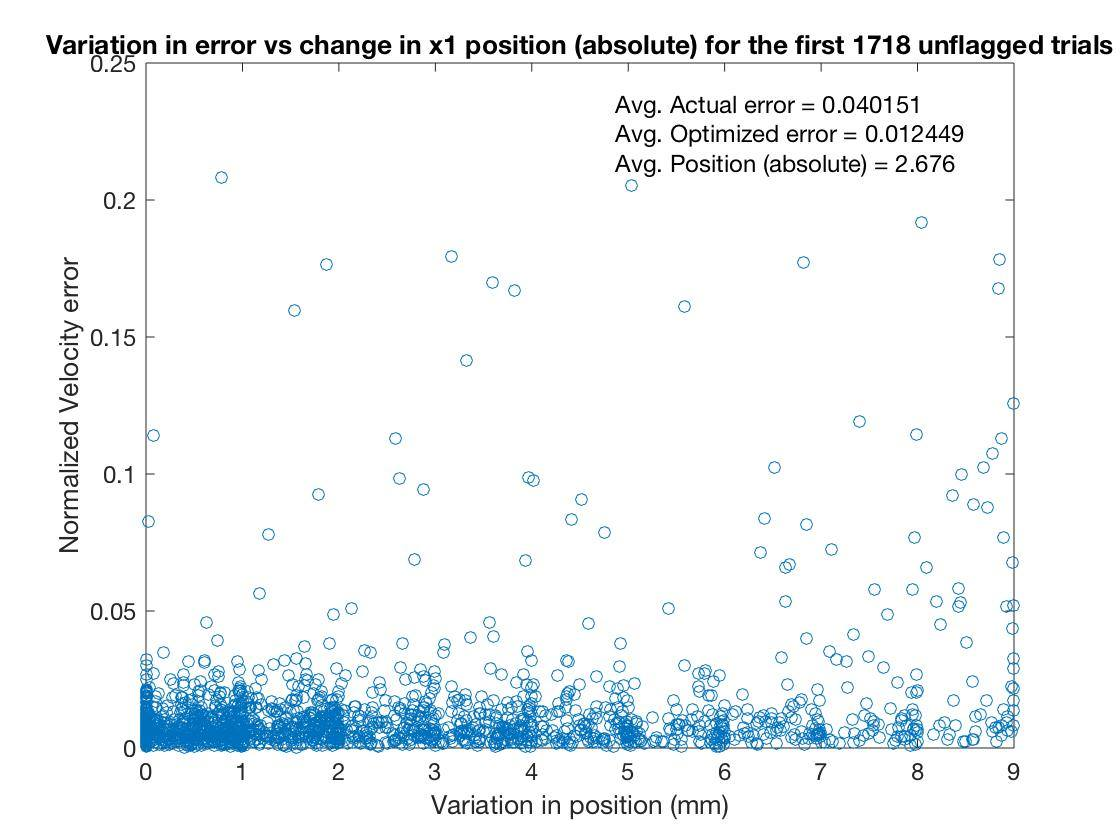
\includegraphics[width=\linewidth]{figures/changeInXPos.jpg}
      \caption{Changing the contact x position in Wang}
      \label{fig:awesome_image1}
    \endminipage\hfill
    \minipage{0.32\textwidth}%
      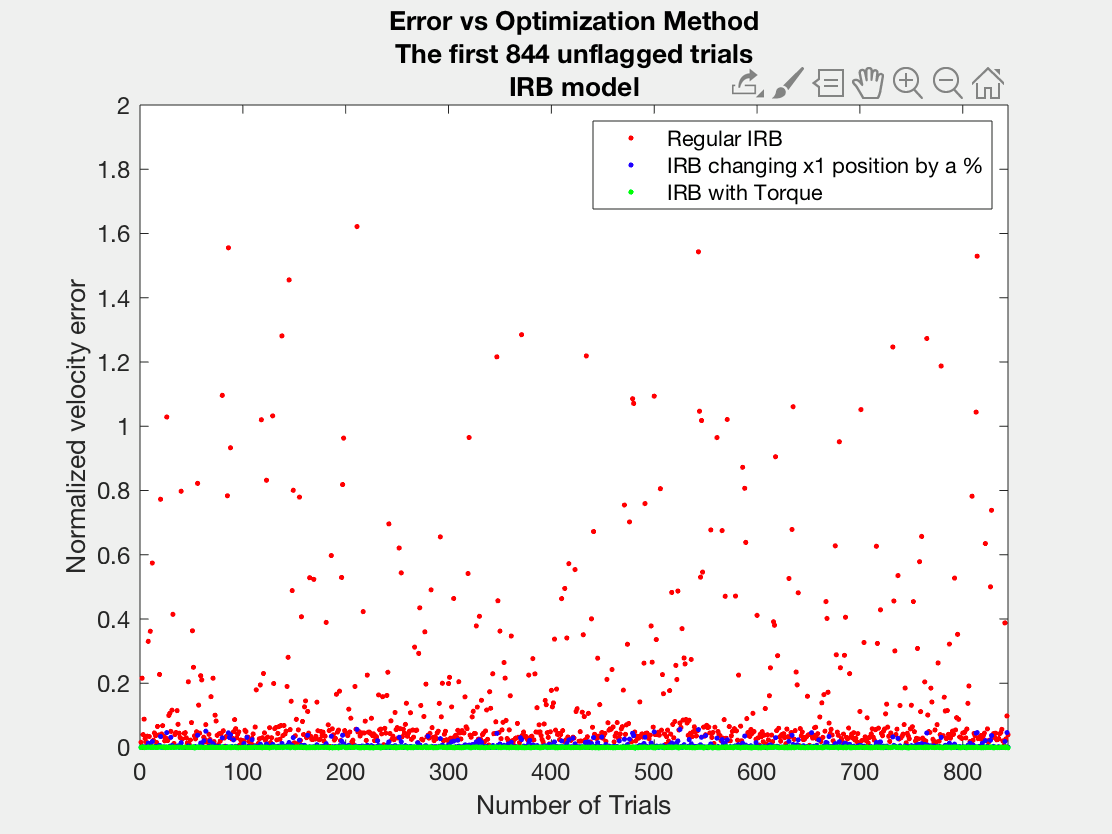
\includegraphics[width=\linewidth]{figures/errorVsOptMethod.png}
      \caption{Changing the contact x position in IRB}
      \label{fig:awesome_image3}
    \endminipage\hfill
    \minipage{0.32\textwidth}
      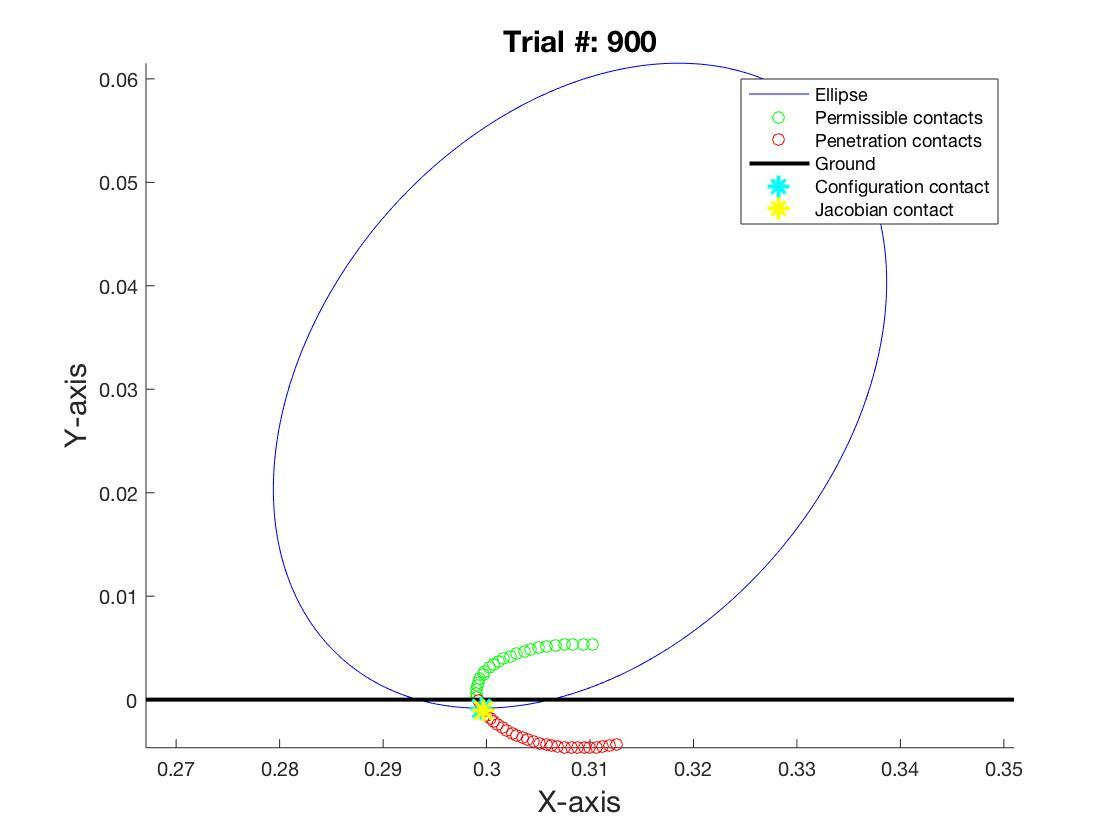
\includegraphics[width=\linewidth]{figures/trial900.jpg}
      \caption{Changing the angle of the ellipse in IRB}
      \label{fig:awesome_image2}
    \endminipage
    \end{figure}        
    
\end{frame}

\begin{frame}{Experiment 1: Errors and Position}
Findings: across all three models, changing by a percentage the positions of the ellipse had a big impact on the accuracy of the results \\
\vspace{\baselineskip}
In general, this is what we saw:
    \begin{itemize}
        \item The measured position already gave a small error (few cases)
        \item Changing the measured position by a little bit gave a large drop in error (most cases)
        \item Changing the measured position by a lot to give a noticeable drop in error (few cases)
    \end{itemize} 
\vspace{\baselineskip}
Conclusion: the data we were provided is not completely accurate!

\end{frame}

%Experiment 2: Errors and Moments
%\subsection{Experiment 2: Errors and Moments}
\begin{frame}{Experiment 2: Errors and Impact Angle}
At first, we were able to find a relationship between the error and the impact angle. 

    \begin{itemize}
%        \item The pre-impact angle is related to both the moment arm and the geometry of the ellipse, which in turn directly affects the torque resulting from the impulse pair
        \item After running our models, we saw a relation between impact angles and the normalized errors (AP and Classic IRB)
        %\item For IRB with torque, the average width (the error offset) was also related to the impact angle.
    \end{itemize} 
\vspace{0.5\baselineskip}
Which means that Some impact angles prevented some of the models from accurately predicting the post-impact states.
    
    \vspace{0.5\baselineskip}
     We will be exploring HOW that link came to be in later slides, but we are still unsure of WHY exactly the models systematically mispredict at certain angles.
\end{frame}

\begin{frame}{Experiment 2: Errors and Impact Angle}
    
 \begin{figure}
 \centering
        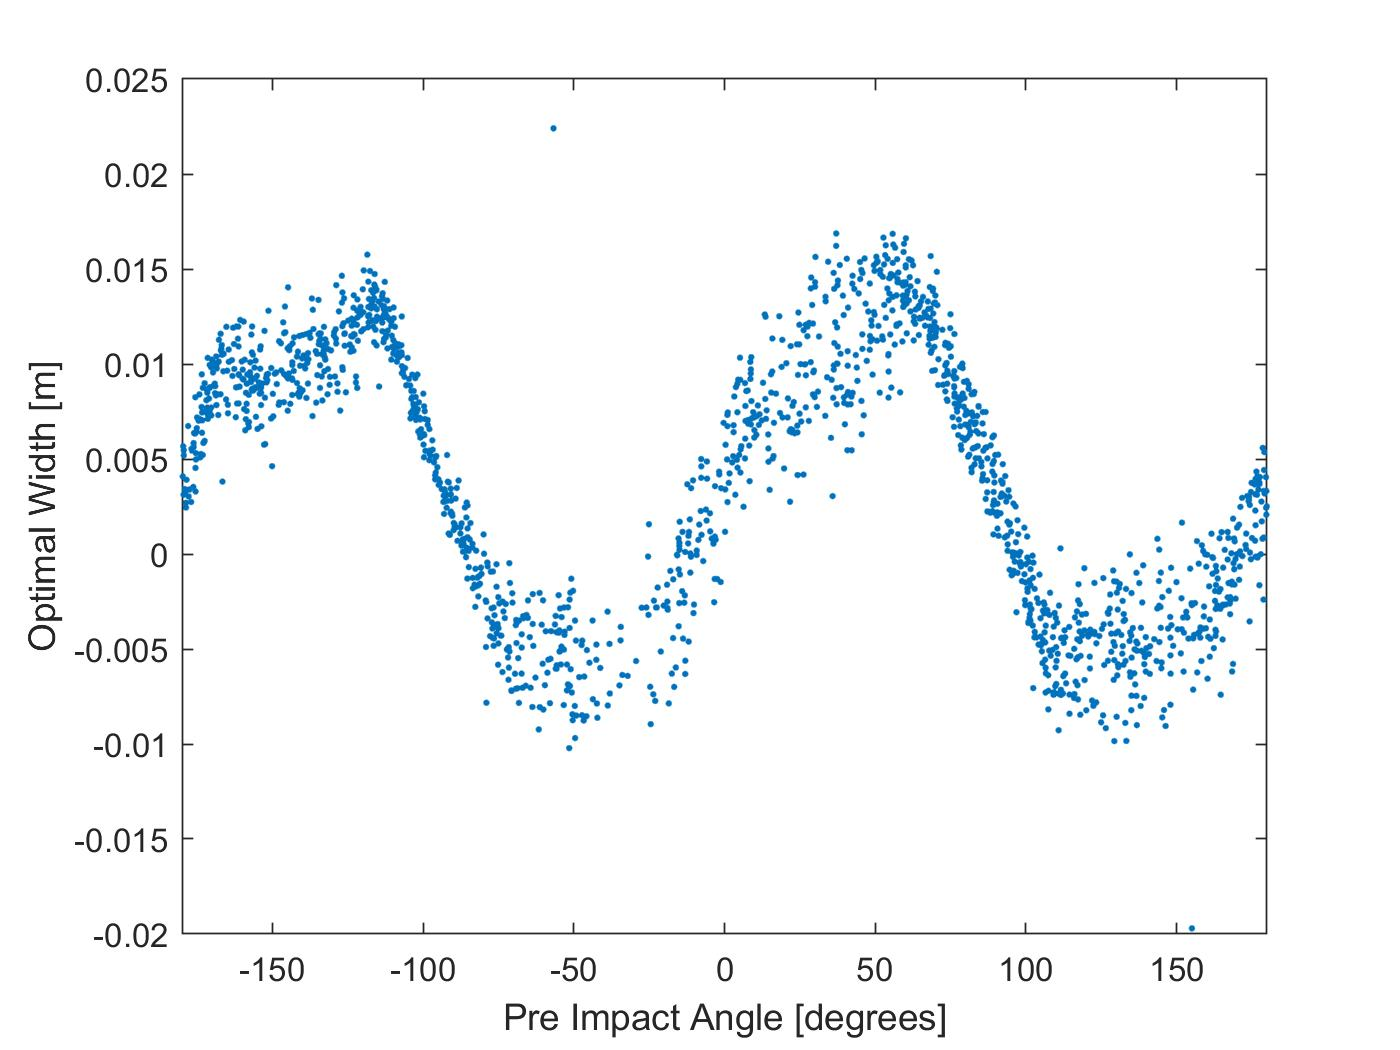
\includegraphics[scale=0.12]{figures/IRBWidthAngle.jpg}
        \caption{IRB With Torque}
        \label{fig:IRBAngle}
\end{figure}
\vspace{-1\baselineskip}

\begin{itemize}
    \item Width can be interpreted as Error
    \item We can see that peaks here occur around -110, -60, 60, 110

\end{itemize}

\end{frame}


\begin{frame}{Experiment 2: Errors and Impact Angle}
\begin{itemize}
    \item Does this trend extend to other models we have looked at?
\end{itemize}

\begin{figure}
    \centering
    \quad
    \begin{subfigure}[b]{0.45\linewidth}
        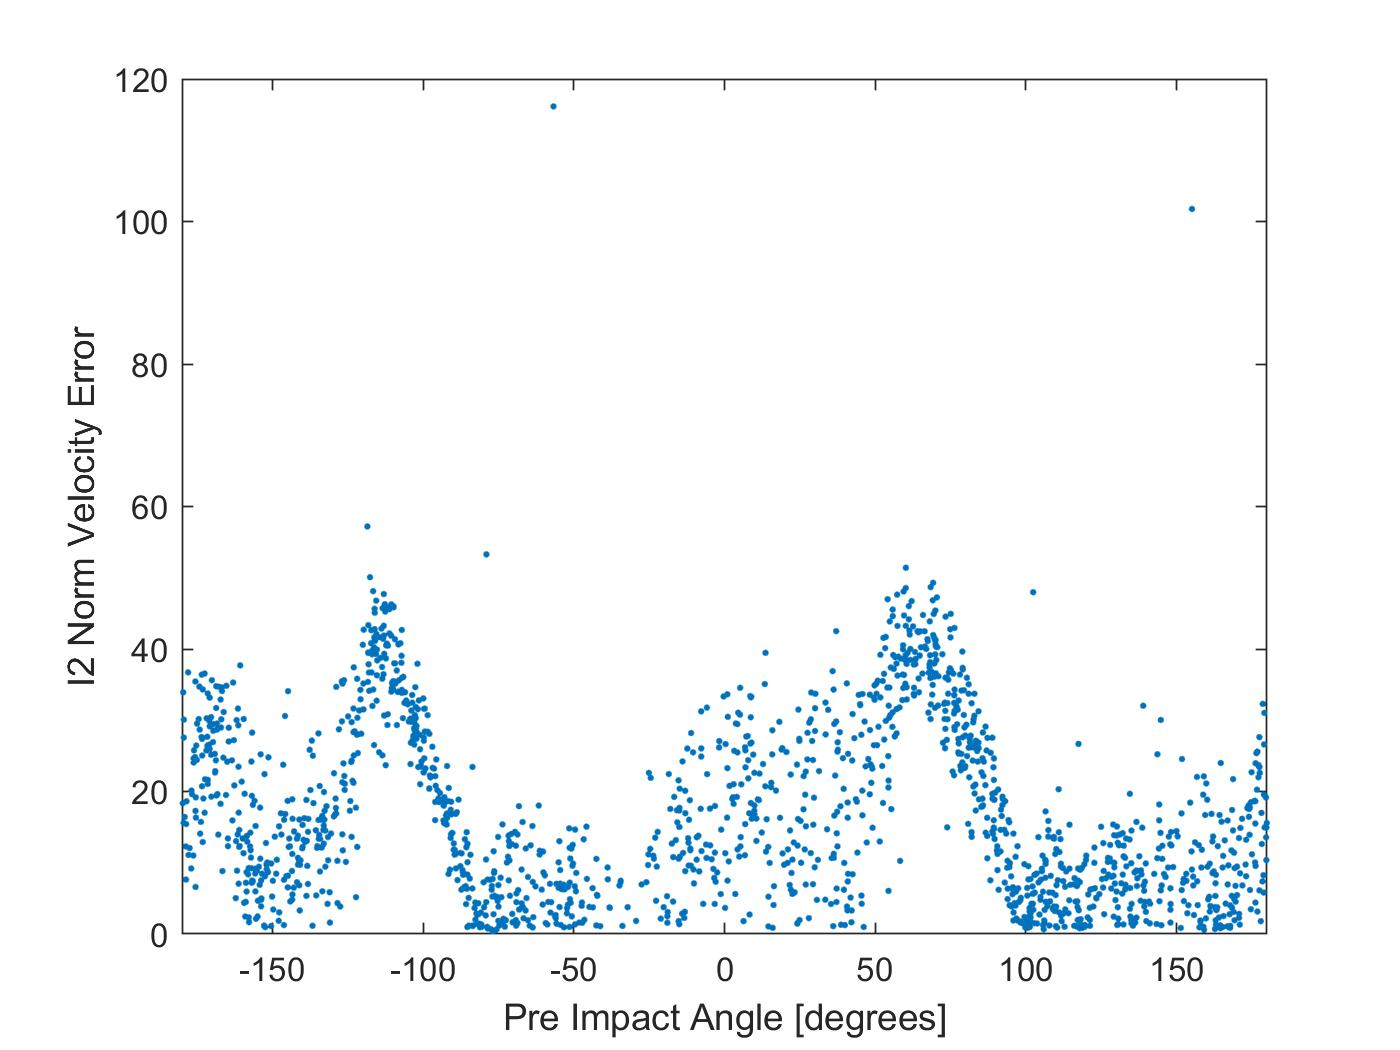
\includegraphics[scale=0.11]{figures/APAngleVsError.jpg}
        \caption{AP Poisson}
        \label{fig:AP_angle}
    \end{subfigure}
    \quad
    \begin{subfigure}[b]{0.45\linewidth}
        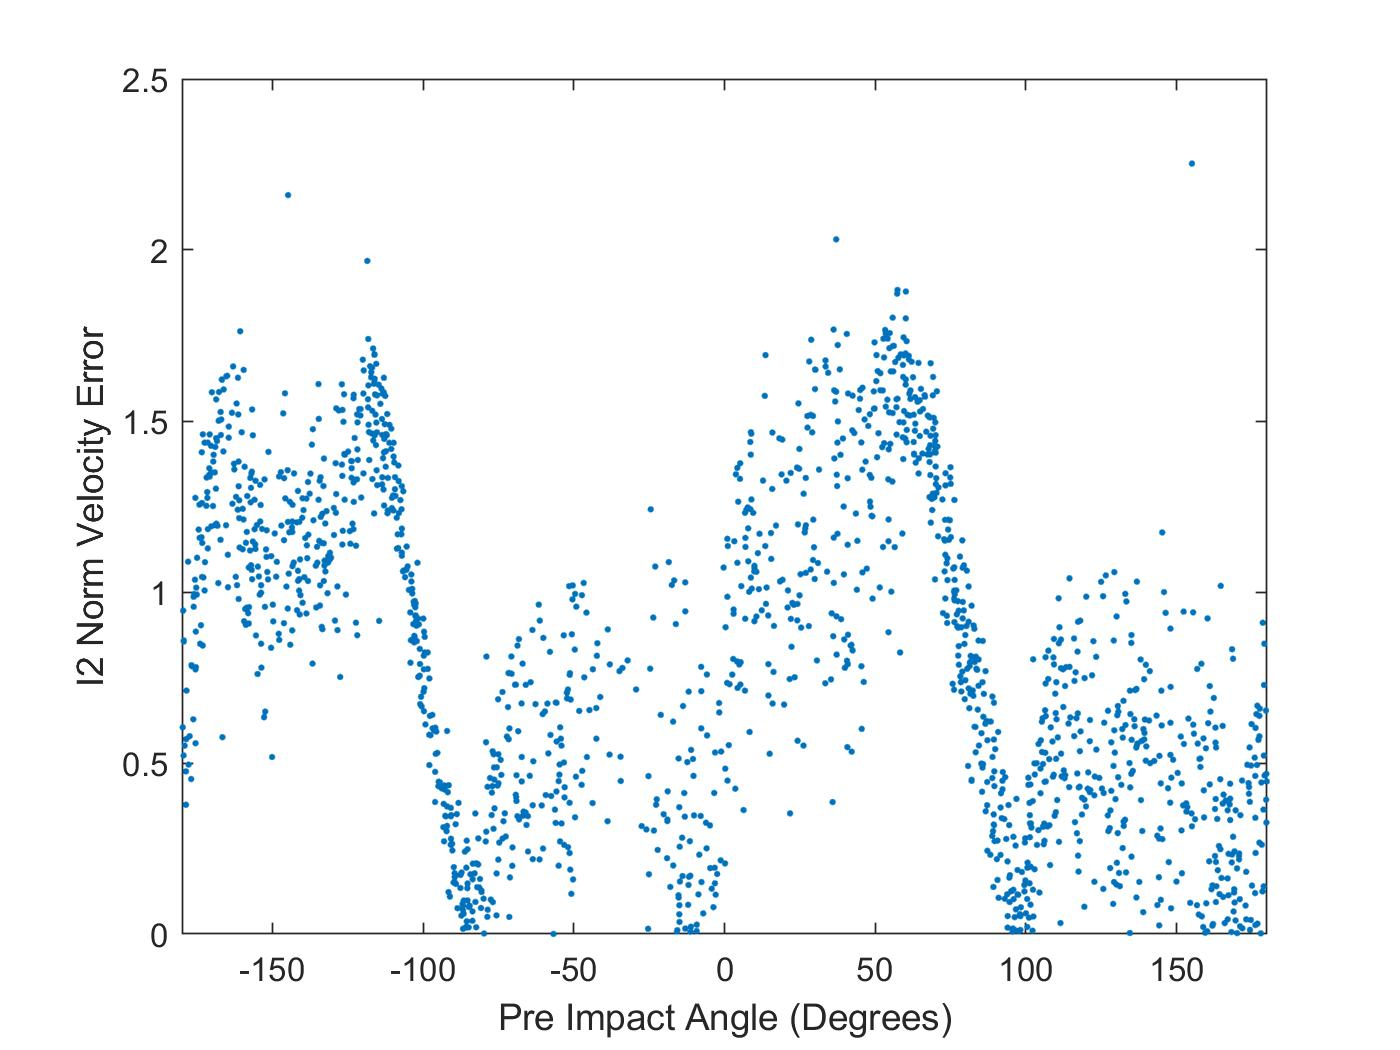
\includegraphics[scale=0.11]{figures/CIRBAngleVsError.jpg}
        \caption{Classical IRB}
        \label{fig:WangAngle}
    \end{subfigure}
\end{figure}
\vspace{-1\baselineskip}

\begin{itemize}
    \item The answer is, kind of!
\end{itemize}

\end{frame}

% \begin{frame}{The Link}

% Overall, this is the link that we have observed between all of our variables
% \vspace{0.5\baselineskip}

% %NEEDS INFO CHECK TO MAKE SURE THIS IS CORRECT

% \begin{itemize}
%     \item  Experiment 3 ($\Delta \dot \theta$ and Impact Angles) - At specific angles, the change in angular velocity is greater than at others. $\Rightarrow$ 
%     \item Experiment 4 ($\Delta \dot \theta$ and Torque) - There is a smaller change in angular velocity at certain angles because at those angles the resultant torque is smaller. $\Rightarrow$ 
%     \item Experiment 5 ($\Delta \dot \theta$ and Errors) - The smaller the change in angular velocity, the greater the prediction error. $\Rightarrow$
%     \item  Experiment 6 (Moments and Errors) - The smaller the Torque, the greater the prediction error. 
% \end{itemize}

% \vspace{0.25\baselineskip}
% %\begin{itemize}
%         %\item In summary: pre-impact angle is related to both the moment arm and the geometry of the ellipse, which in turn directly affects the torque resulting from the impulse pair
%         In summary: At specific angles, there are smaller resultant torques, and at these smaller resultant torques, the prediction error of the IRB model is greater.
%     %\end{itemize} 

% \end{frame}


%Experiment 3: Impact angles and Change in angular velocity
\begin{frame}{Experiment 3: $\Delta \dot \theta$ and Impact Angles}

\begin{itemize}
    \item We expected the ellipse to have a greater change in angular velocity if it didn't fall right on its center of mass.
    \item The greater the moment arm, the greater the change in angular velocity.
\end{itemize}
\begin{figure}
    \centering
    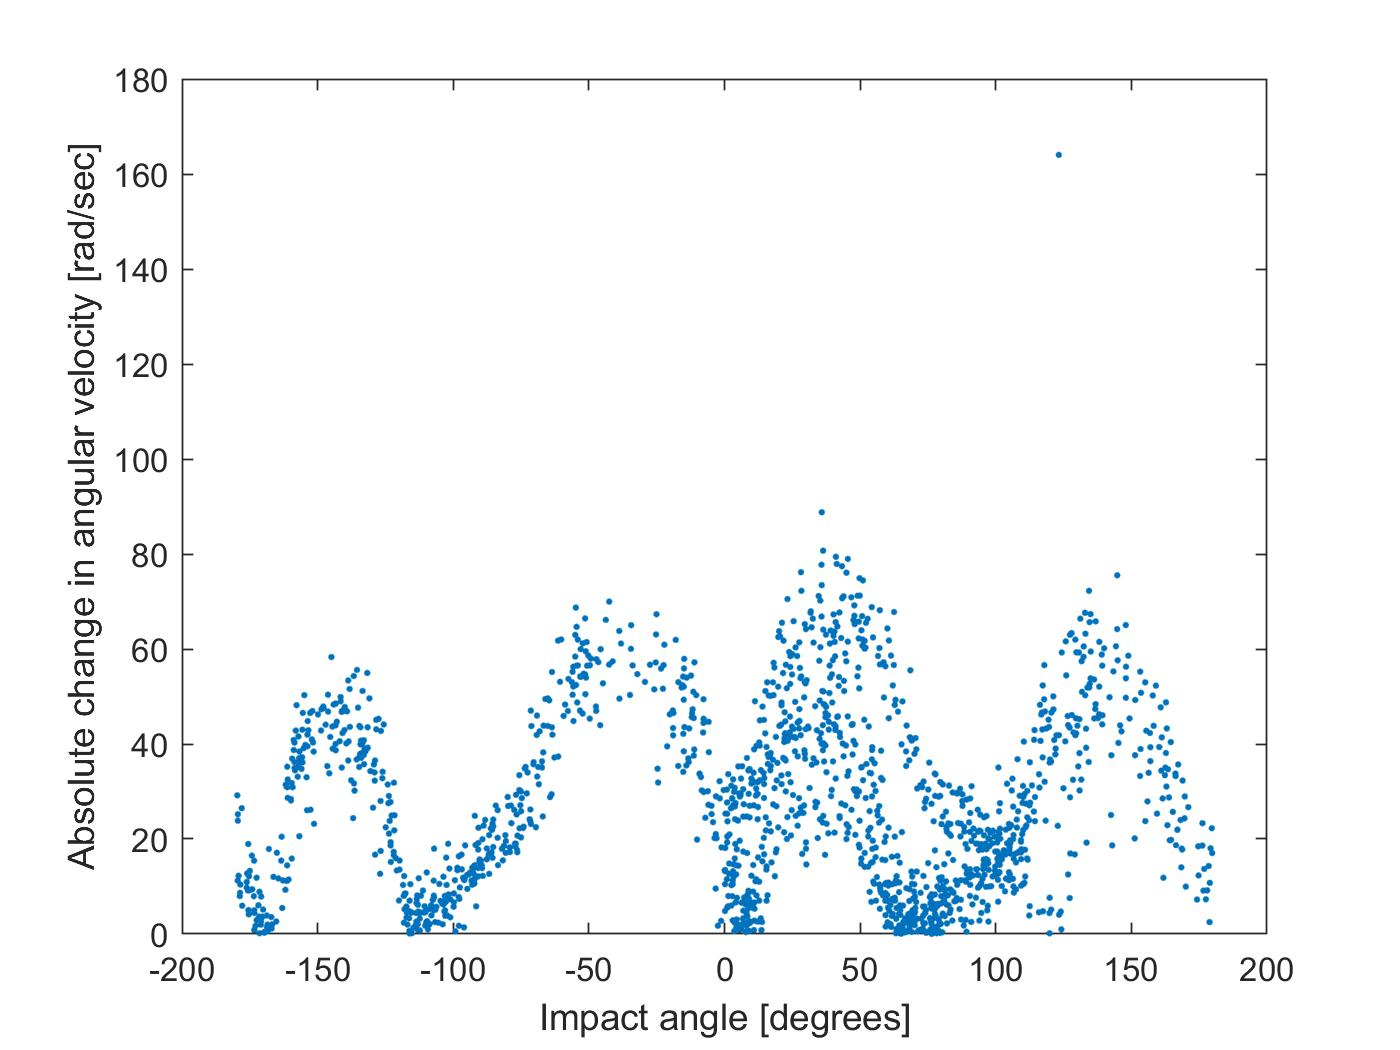
\includegraphics[scale=0.12]{figures/impact angle vs change in angular velocity.jpg}
    \caption{All moments vs Error}
    \label{fig:MomentsError}
\end{figure}
\item At around -110, 60, 110 the change in angular velocity is close to 0.
\end{frame}

%Experiment 4: Change in angular velocity and Torque
\begin{frame}{Experiment 4: $\Delta \dot \theta$ and Torque}
%this kind of ties in to the previous slide/it's already been said that greater change in angular velocity leads is related to greater moment/torque so maybe just delete this one?

\begin{figure}
    \centering
    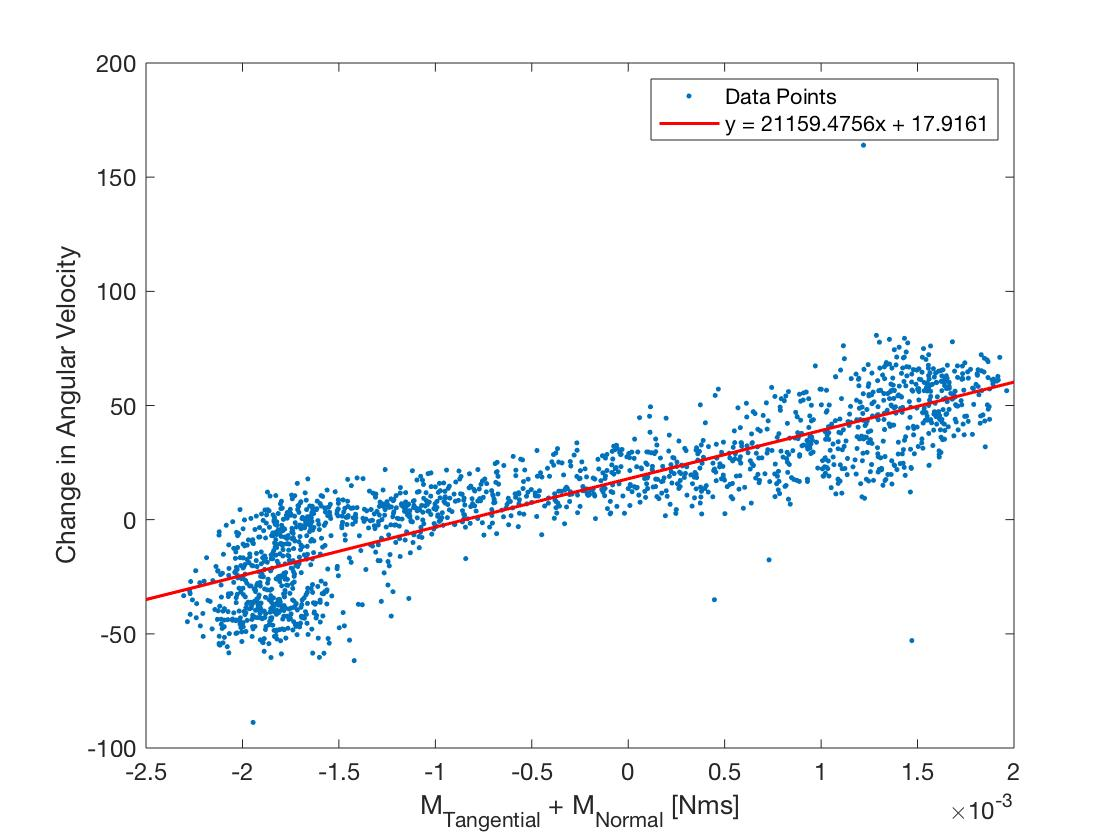
\includegraphics[scale=0.21]{figures/AngularVvsMoment.jpg}
    \caption{Classic IRB: Change in Angular Velocity vs Total Moment}
    \label{fig:MomentsError}
\end{figure}

\end{frame}

%Experiment 5: Link between angular velocity and error
\begin{frame}{Experiment 5: $\Delta \dot \theta$ and Errors}

\begin{figure}
    \centering
    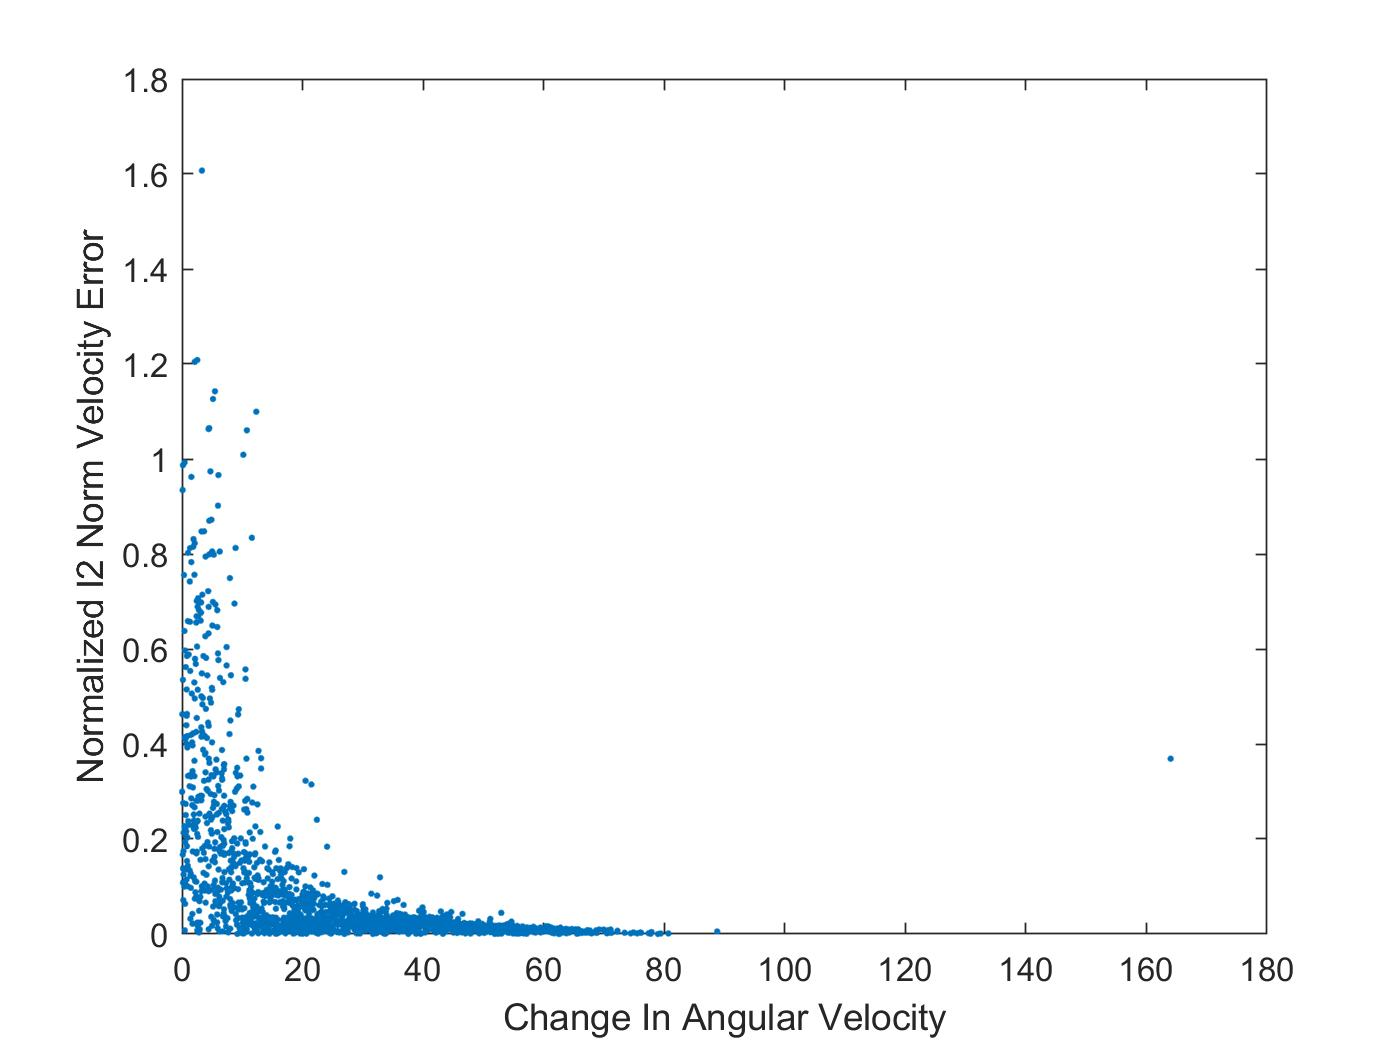
\includegraphics[scale=0.17]{figures/changeInOmegaEllipse.jpg}
    \caption{Classic IRB: Change in Angular Velocity vs Error}
    \label{fig:AngularVError}
\end{figure}
\end{frame}

%The important part about this slide is the idea of overcompensation. The width isn't just helping adjust for changes in angular velocity that are too large for the IRB to predict and need more torque.... It is allowing for the IRB to change the impulses and create large torques/changes in omega which the width can then cancel out potentially 

%Experiment 6: Link between Moments and Error [editttttttt]
\begin{frame}{Experiment 6: Moments and Errors}

% Since a greater angular velocity change led to a smaller error, and the angular velocity change is directly related to the net torque, As a sanity check, we graphed the net torque vs the normalized error hoping to see the same trend.

%\vspace{0.25\baselineskip} [PRESENTATION NOTES]
%The difference between these next 2 plots is the magnitude of the normalized error. IRB torque has a minor error magnitude compared to the classical model, because the compression width applies a moment to "Correct" the angular velocity.
 
\begin{figure}
    \centering
    \quad
    \begin{subfigure}[b]{0.4\linewidth}
        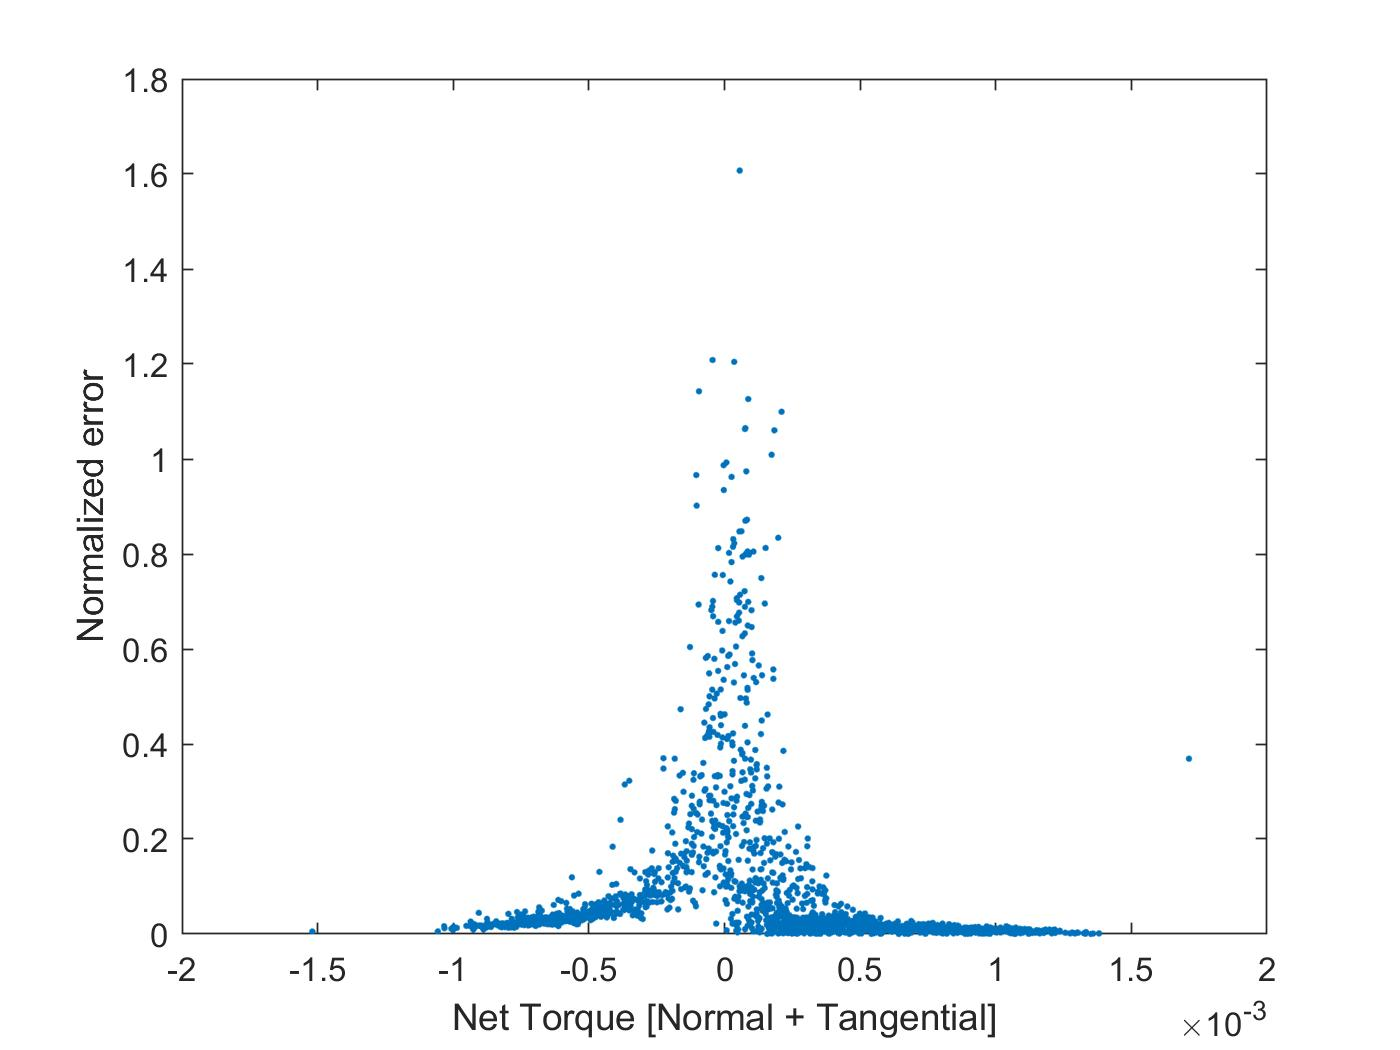
\includegraphics[scale=0.105]{figures/IRB Classic Net torque vs error.jpg}
        \caption{Net Torque vs Error}
        \label{fig:AP_angle}
    \end{subfigure}
    \quad
    \begin{subfigure}[b]{0.5\linewidth}
        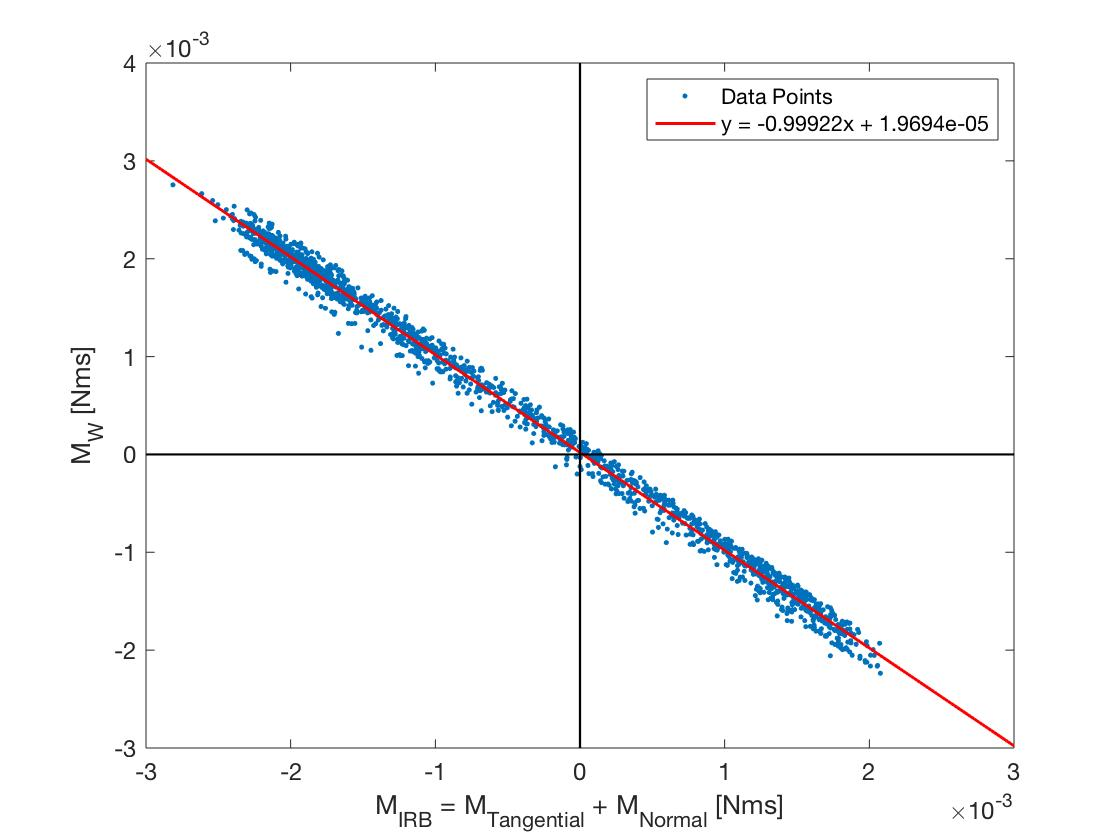
\includegraphics[scale=0.13]{figures/MomentProp2.jpg}
        \caption{IRB Moment vs Torque}
        \label{fig:MomentIRB}
    \end{subfigure}
\end{figure}    
    
    
\end{frame}

\begin{frame}{The Link}

\tikzstyle{startstop} = [rectangle, rounded corners, minimum width=2.5cm, minimum height=1.75cm, text centered, text width = 4cm, draw=black]
\tikzstyle{arrow} = [thick,->,>=stealth]
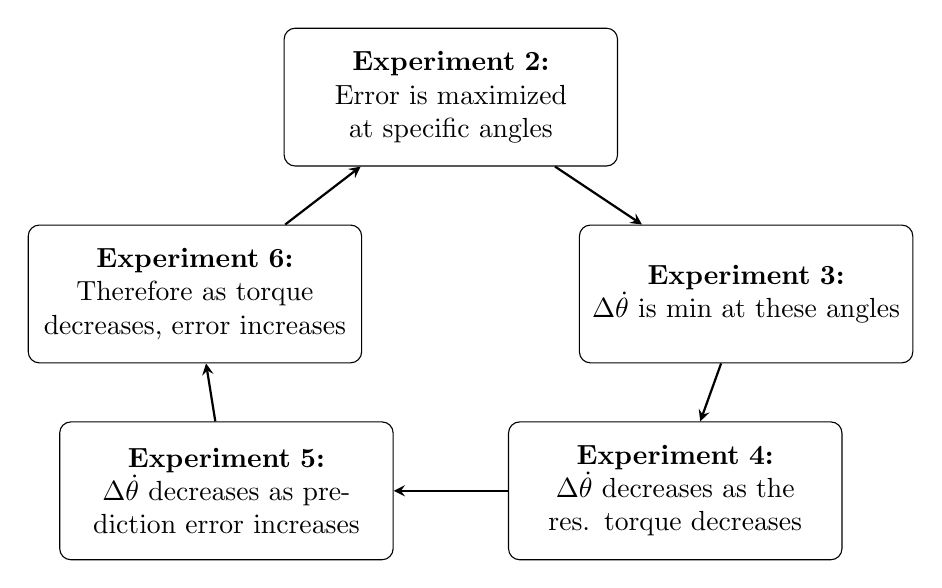
\begin{tikzpicture}[node distance=2cm]

\node (exp2) [startstop, xshift = 3.5cm, yshift = 11cm] {\textbf{Experiment 2:} \\ Error is maximized at specific angles};
\node (exp3) [startstop, xshift = 7.25cm, yshift = 8.5 cm] {\textbf{Experiment 3:} \\ $\Delta \dot \theta$ is min at these angles};
\node (exp4) [startstop, xshift = 6.35cm, yshift = 6cm] {\textbf{Experiment 4:} \\  $\Delta \dot \theta$ decreases as the res. torque decreases};
\node (exp5) [startstop, xshift = 0.65cm, yshift = 6cm] {\textbf{Experiment 5:} \\ $\Delta \dot \theta$ decreases as prediction error increases};
\node (exp6) [startstop,xshift = 0.25cm, yshift = 8.5cm] {\textbf{Experiment 6:} \\ Therefore as torque decreases, error increases};


\draw [arrow] (exp3) -- (exp4);
\draw [arrow] (exp4) -- (exp5);
\draw [arrow] (exp5) -- (exp6);
\draw [arrow] (exp6) -- (exp2);
\draw [arrow] (exp2) -- (exp3);

\end{tikzpicture}
\end{frame}
